\input sys/inputs.tex

\begin{document}

\bigheading{Critical Projects}

% \info{task_name}{infile}{outfile}{points}{timelimit}{memlimit}
% leave this values, if you are not interested
\info{critical}{stdin}{stdout}{100}{600 ms}{32 MiB}

A large project is subdivided into $N$ different subprojects. The manager of the project established precedence relations among the subprojects. This means that there are pairs of subprojects $u$ and $v$ such that the completion of the subproject $u$ must be finished before the start of the subproject $v$. In this case we say that $u$ directly precedes $v$. We say that $u$ precedes $v$ if $u$ directly precedes $v$ or there is a subproject $z$ such that $u$ precedes $z$ and $z$ precedes $v$.
Any subproject $u$ is considered critical if for each subproject $v$ (other than $u$) either $v$ precedes $u$ or $u$ precedes $v$. It is known that the whole project can be completed, e.i., there is no subproject $u$ such that $u$ precedes itself.

\heading{Task}
Write a program that computes all the critical subprojects.

\heading{Input}
The first line of the input contains two integers, $N$ and $M$. $N$ ($1 \leq N \leq 100000$) is the number of the subprojects and $M$ ($0 \leq M \leq 1000000$) is the number of the direct precedence pairs. Subprojects are identified by the numbers $1, \ldots ,N$. Each of the next $M$ lines contains two integers $u$ and $v$, ($1 \leq u \neq v \leq N$) a direct precedence pair, that is $u$ directly precedes $v$.\\
\bigskip
In $40 \%$ of the testcases $N \leq 5000$ and $M \leq 30000$ also hold.

\heading{Output}
The first line of the output must contain the number of critical subprojects. The second line contains the identifiers of the critical subprojects in ascending order. The numbers must be separated by a single space. If there is no critical subproject then the first and only line contains the number 0.

\heading{Samples}

\sampleIN
7 9
1 3
2 3
3 4
3 5
4 6
5 6
1 7
3 7
7 4
\sampleOUT
2
3 6
\sampleCOMMENT

\sampleEND

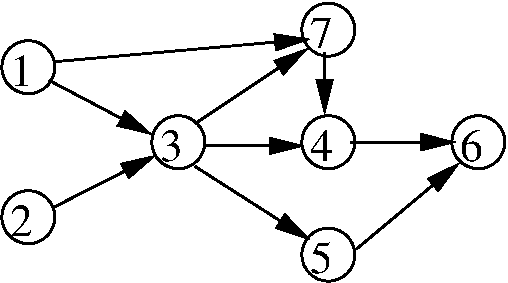
\includegraphics[height=4cm]{img/critical-fig.pdf}
\bigskip


\end{document}
